% !TeX root = ../../thesis.tex

\subsubsection{Descriptive Statistics}
The number of samples varied across the hospitals, ranging from 2364 to 18177. Distributions of the selected variables are presented in table \ref{tab:obs_material_1}. The sum of all samples totals 73351.

\begin{table}[htbp]
  \centering
  \caption[Distribution of features used for prediction of delivery Type]{Distribution of features used for prediction, Mean and Standard Deviation (SD) for continuous variables. Mode and percentage for categorical variables. Number of samples is 73351.}
  \label{tab:obs_material_1}
   \renewcommand{\arraystretch}{1.02} % Adjust the vertical spacing
  \setlength{\tabcolsep}{12pt} % Adjust the horizontal spacing
    \begin{tabular}{m{15em}cc}
    \toprule
        Variable & M (SD) & Mode [\%] \\ 
        \hline
        Mother Age & 31.0 (5.6) & ~ \\ 
        Weight pre-pregnancy & 65.8 (13.9) & ~ \\ 
        Weight on admission & 78.6 (14.2) & ~ \\ 
        \ac{bmi} & 25.0 (5.4) & ~ \\ 
        Previous eutocic delivery & 0.4 (0.7) & ~ \\ 
        Previous vacuum-assisted delivery & 0.1 (0.3) & ~ \\ 
        Previous forceps & 0.0 (0.1) & ~ \\ 
        Previous \ac{cs} & 0.1 (0.4) & ~ \\ 
        Fetal presentation on admission & ~ & cephalic [26.323\%] \\ 
        Bishop score & 5.5 (3.0) & ~ \\ 
        Gestational age on admission & 38.9 (1.9) & ~ \\ 
        Premature rupture of the membrane & ~ & No [87.991\%] \\ 
        Chronic hypertension & ~ & No [97.676\%] \\ 
        Gestational hypertension & ~ & No [97.749\%] \\ 
        Preeclampsia & ~ & No [98.299\%] \\ 
        Gestational diabetes & ~ & No [89.811\%] \\ 
        Gestational diabetes treated with diet & ~ & No [94.285\%] \\ 
        Gestational diabetes treated with insulin & ~ & No [98.083\%] \\ 
        Gestational diabetes treated with oral antidiabetic drugs & ~ & No [97.797\%] \\ 
        Maternal Diabetes & ~ & No [99.509\%] \\ 
        Type 1 Diabetes & ~ & No [99.816\%] \\ 
        Type 2 Diabetes & ~ & No [99.843\%] \\ 
        Presentation at birth & ~ & Vertex presentation [94.000\%] \\ 
        Delivery & ~ & Spontaneous [53.864\%] \\ 
        Gestational age on birth & 39.0 (1.8) & ~ \\ 
        Smoking during pregnancy & ~ & No [88.442\%] \\ 
        Alcohol consumption during pregnancy & ~ & No [98.65\%] \\ 
        Consumed drugs during pregnancy & ~ & No [99.825\%] \\ 
        Nr of pregnancies (with current) & 1.9 (1.1) & ~ \\ 
        Pregnancy type & ~ & Spontaneous [85.417\%] \\ 
        Surveillance & ~ & yes [97.699\%] \\ 
        Hospital surveillance & ~ & yes [67.807\%] \\ 
        Pelvis Adequacy & ~ & Adequate [17.512\%] \\ 
        Consistency of the cervix & 1.6 (0.6) & ~ \\ 
        Fetal station & 0.8 (0.8) & ~ \\ 
        Dilation of the cervix & 1.3 (0.8) & ~ \\ 
        Effacement of the cervix & 1.2 (1.2) & ~ \\ 
        Position of the cervix & 0.6 (0.7) & ~ \\ 
        Haematologic disease & ~ & No [95.674\%] \\ 
        Respiratory disease & ~ & No [95.605\%] \\ 
        Cerebral disease & ~ & No [98.793\%] \\ 
        Cardiac disease & ~ & No [92.967\%] \\ 
        Neuroaxis techniques & ~ & 1 [69.5\%] \\ 
        Number of children  & 0.6 (0.8)  & ~\\ 
        \bottomrule
    \end{tabular}


\end{table}
The outcome variable had the following distribution as stated in table \ref{tab:delivery_methods}.

\begin{table}[htbp]
  \centering
  \caption{Distribution of Delivery Methods}
  \label{tab:delivery_methods}
  \renewcommand{\arraystretch}{1.5} % Adjust the vertical spacing
  \setlength{\tabcolsep}{12pt} % Adjust the horizontal spacing
  \begin{tabular}{lc}
    \hline
    \textbf{Type of delivery} & \textbf{Frequency (\%)} \\
\hline
    \ac{cs} & 19 803 \, (27\%) \\

    Vaginal & 38 189 \, (52\%) \\

    Instrumental delivery & 15 359 \, (21\%) \\
    \hline
  \end{tabular}
\end{table}
%Vaginal      0.520634
%Cesariana    0.269976
%auxiliado    0.209390



\subsubsection{The Model}
The \ac{auroc} is presented in table \ref{tab:performancemetricsauc} for the best hyper-parameters found for each algorithm in the training data. All models used the variables indicated in table \ref{tab:obs_material_1}.
\begin{table}[htbp]
  \centering
  \caption[Performance Metrics in the training set]{Repeated Cross-validation (10x2) results in the training set with mean AUROC and 95\% Confidence Interval (CI) for best hyper-parameters found for each algorithm. Wilcoxon Test for comparing with the best performing algorithm.}
  \label{tab:performancemetricsauc}
  \renewcommand{\arraystretch}{1.5} % Adjust the vertical spacing
  \setlength{\tabcolsep}{12pt} % Adjust the horizontal spacing
  \begin{tabular}{lccc}
    \hline
    \textbf{Metric} & \textbf{AUROC} & \textbf{CI 95\%} \textit{\textbf{P value}} \\
    \hline
    XGBoost & 0.8809 & 0.8799, 0.882 & - \\  
    Decision Tree & 0.8337 & 0.8324, 0.8349 & $\leq$ 0.001\\
    Logistic Regression & 0.8716 & 0.8706, 0.8726 & $\leq$ 0.001\\
    AdaBoost & 0.8753 & 0.874, 0.8766 & $\leq$ 0.001\\ 
    lightgbm & 0.8805 & 0.8793, 0.8817 &  0.003\\ 
    Stochastic Gradient Descent & 0.8704 & 0.8694, 0.8713& $\leq$ 0.001\\ 
    Random Forest & 0.8752 & 0.8743, 0.8762& $\leq$ 0.001 \\  
    \hline
  \end{tabular}
\end{table}
While XGBoost was the best-performing algorithm, we selected LightGBM  \cite{lightgbm} because of its speed and lower memory requirements, which we believe are better suited for deployment in a low-hardware environment. The threshold selected for deploying the model was 0.7457 which rendered the metrics in the test set, as shown in table \ref{tab:performancemetricsthreshold}.

\begin{table}[htbp]
  \centering
\caption{Performance Metrics in the test set with chosen threshold}
\label{tab:performancemetricsthreshold}
\renewcommand{\arraystretch}{1.5} % Adjust the vertical spacing
\setlength{\tabcolsep}{12pt} % Adjust the horizontal spacing
\begin{tabular}{lc}
    \hline
    \textbf{Metric} & \textbf{Value} \\
    \hline
    Accuracy & 0.8052 \\
    Sensitivity & 0.8223 \\
    Precision & 0.9023 \\
    F1 Score & 0.8605 \\
    \hline
  \end{tabular}
\end{table}




\subsubsection{Deployment}
The purpose of this model is to serve as an \ac{api} for usage within a healthcare institution and to act as a supplementary clinical decision support tool for obstetrics teams. For this to happen, a health information system must make the requests to the API. Even though a concrete, vendor-specific information model and input health information system were used, we hope to create a more interoperable clinical decision support system that can be used by every system that acts on birth and obstetrics departments. Therefore, we built it around the \ac{hl7} \ac{fhir} standard (R5 version) to simplify the method of interacting with the \ac{api}. This decision, opposed as to using a proprietary model for the data, sits upon the usage of \ac{fhir} resources: Bundle and Observation for request and returning the result as a message through a custom operation called "\$predict". It is intended to publish the profiles of these objects in order to facilitate access to the \ac{api} using standardized mechanisms and data models. The current build of the profiles can be seen in the published \ac{fhir} Implementation Guide where the current specifications are described in detail \url{https://joofio.github.io/obs-cdss-fhir/}. The process is illustrated in figure \ref{fig:deploy}. We deployed this model in production in a single hospital without a user interface, collecting only the data and predictions for later discussion and analysis. We collected 3231 requests. During this period, 123 (3.8\%) alarms were triggered. From this, we tried to understand the level of certainty for the decision and check the difference from the threshold of these alarms. The distance to the threshold for 73 was lower than 0.1 and was bigger than 0.1 for 50 (1.55\%) cases.


%TC:ignore

\begin{figure}[htbp]
\centering
\captionsetup{justification=centering}
\caption{Deployment and decision mechanism of the model}\label{fig:deploy} 
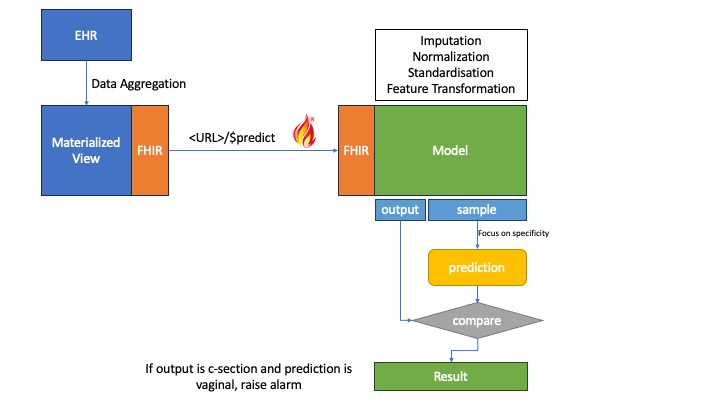
\includegraphics[scale=0.60]{figures/obs-model.jpg}
\end{figure}
%TC:endignore

\subsubsection{Clinical Evaluation}
The median scores given by each clinician are presented in figure \ref{fig:clinical}. We also predicted the result using our model as stated in figure \ref{fig:clinical}. The model misclassified only one record (4). As for the analysis of missing features for the responders, they were divided into 3 categories: 1) Existent in the dataset but not included in the model, 2) Non-existent in the dataset and 3) existent in the dataset and included but that particular information was not filled for the patient assessed. This rendered a total of 62 \% non-existent and 38 \% existent but no information was provided at that moment. No feature mentioned existed in the dataset but had not been included in the model. From the non-existent, 38 \% were new clinical assessments, 38\% were linked to information from previous births, 15\% connected in more in-depth information about provided information (i.e, motive for induction) and 11\% were related to the mother's choice (if she wanted a C-section). As for feature importance, from the 60 answers, we got 55 \% with labor being the most important factor. 15 \% answered the number of previous vaginal births, 8 \% the evolution of weight and another 8\% the number of previous C-sections. The remaining 14\% were various features, from BMI, neuroaxis techniques, gestational age and weight of the mother. Of all of these, 90 \% were in the top 10 features of the model.



%TC:ignore

\begin{figure}[htbp]
\centering
\captionsetup{justification=centering}
\caption[Obstetrics questionnaires data]{Validation data. The colour represents the actual birth type. The boxplot represents the median and \ac{iqr} of the reviewers and the X represent each patient case. Contains 6 Vaginal births and 4 \acp{cs}. * represents wrong predictions of the model. (ID: 4)}\label{fig:clinical} 
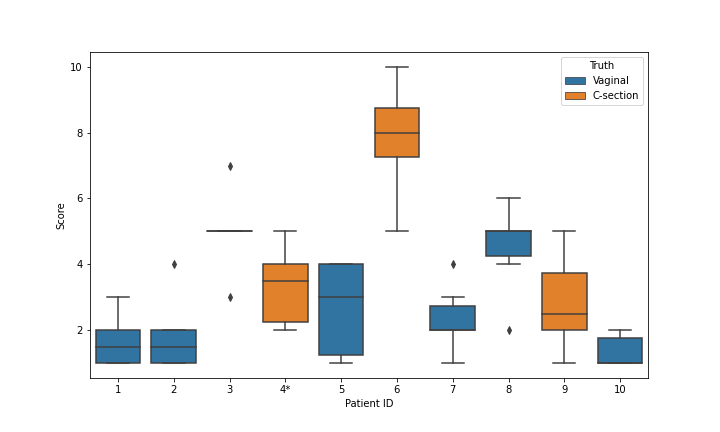
\includegraphics[scale=0.60]{figures/clinical_assessment.png}
\end{figure}
%TC:endignore




\subsubsection{Potential Financial Impact}
The financial support provided to public hospitals in Portugal is partially tied to the rate of C-sections. To assess the potential impact of this mechanism on Portuguese public hospitals, we conducted a simulation. We got data for every public hospital for the last 12 months and applied a 3.8\% reduction (the rate of warnings triggered in the new dataset) and recalculated the rate of C-sections. The increase in support was calculated by the state-mandated rate as shown in table \ref{tab:corrections}. With this new rate, we observed that implementing our tool would result in financial benefits for 30\% (11 hospitals) of the public hospitals. Specifically, five hospitals would begin receiving support instead of no support at all. Three hospitals would experience a doubling of their financial benefit, while two hospitals would see a 50\% increase. Furthermore, one hospital would receive an additional one third of financial support. If we assumed that only half of the warnings found in the new data were actually true (1.9\%) we found that only 6 hospitals would be benefited. 3 from 0 to 0.25, 2 from 0.25 to 0.50 and 1 from 0.50 to 0.75.


\begin{table}[htbp]
  \centering
  \caption[Ruleset for financial support indexed to \acsp{cs}.]{Ruleset for state-provided financial support indexed to \acp{cs}. X is the current payment of a \ac{cs} inpatient episode. Adapted from \cite{acssTermosReferenciaPara2023}}
  \label{tab:corrections}
  \renewcommand{\arraystretch}{1.2} % Adjust the vertical spacing
  \setlength{\tabcolsep}{12pt} % Adjust the horizontal spacing
  \begin{tabular}{lc}
      \hline
Rate of \acp{cs}   & Support \\
    \hline
\textless 25\%       & x       \\
{[}25\%, 26.4\%{]}   & 0.75 x   \\
{[}26.5\%, 27.9\%{]} & 0.5 x    \\
{[}28\%, 29.4\%{]}   & 0.25 x   \\
\textgreater{}29.5\% & 0      \\
    \hline
\end{tabular}
\end{table}